\documentclass[10pt,a4paper,fleqn]{article}
\usepackage[margin=20mm]{geometry}
\usepackage{fontspec}

\usepackage{amsmath} %math package
\usepackage{amsfonts} %math package
\usepackage{amssymb} %math package
\usepackage{gensymb} %math symbol package
\usepackage{graphicx} %graphic package
\usepackage{fancyhdr} %pagestyle package
\usepackage{xcolor} %color package aiming to change color of text
\usepackage{adjmulticol} %able to use multicols environment

\pagestyle{fancy}
\fancyhead{}
\fancyfoot[c]{\thepage}
\renewcommand{\headrulewidth}{0pt} %header line thickness
\parindent 0ex %paragraph indentation

\def\bslash{\textbackslash} %Macro, you can indicate a name for a cammand
\def\d{\displaystyle}

\begin{document}
\title{\Huge \textbf{Basic \LaTeX}}
\author{NG KANG NANG}
\date{}
\maketitle 
\vfill %verticle space
\tableofcontents
\vfill
\pagebreak

\section*{Before Start}
You need some preparations before starting to use \LaTeX.
\subsection*{1. Install MiKTeX or MacTeX}
For Windows users, you are suggested to install MiKTeX. For MacOS users, you are suggested to install MacTeX.
\subsection*{2. Install Texmaker}
Texmaker is a good Tex editor for beginners.
\subsubsection*{\quad 2.1 Setup Texmaker}
\clearpage
\section*{Packages List}
\begin{multicols}{3}
{\large \textbf{Common packages} }\\[1mm]
1. fontenc: do not import for XeLaTeX!\\
2. inputenc: do not import for XeLaTeX!\\
3. babel\\
4. setspace\\
5. fancyhdr\\
6. textcomp: import before ``gensymb'' to prevent warning in latex but \textit{do not import for XeLaTeX} \\
7. graphicx\\
8. xcolor\\
9. adjmulticol\\
10. wrapfig\\
11. subcaption\\
12. array
\columnbreak

{\large \textbf{Maths packages} }\\[1mm]
1. gensymb\\
2. amsmath\\
3. amssymb\\
4. amsfonts
\columnbreak

{\large \textbf{Packages for XeLaTeX} }\\[1mm]
1. fontspec\\
2. xeCJK\\
3. Do not import ``textcomp''
\end{multicols}

\section*{XeLaTeX}
XeLaTeX is different from LaTeX and pdfLaTeX since it directly read UTF-8. So, it is important to remember to set the compiler encoding into UTF-8.

It is convenient to use ``xecjk'' package to output Chinese in XeLaTeX. It is suggested to use XeLaTeX as main tool if you need to output Chinese
\pagebreak

\section{Basic Document Structure}
\bslash documentclass\{article\}\\
\textit{preamble}\\
\bslash begin\{document\}\\
\textit{content}\\
\bslash end\{document\}

\section{How to make a title page}
You can make a title page by using environment: ``\bslash begin\{titlepage\}'',
or you can just use``\textbackslash maketitle'', while it will leave the page number at the footage. If you use `titlepage' environment, you will be able to adjust the page style.

\section{Basic Skills}
\subsection{Basic Commands}
\begin{enumerate}
\item spacing: (\quad): quad(\bslash quad), (\,): 3/18 quad(\bslash ,), (\:): 4/18 quad(\bslash :), (\;): 5/18 quad(\bslash ;), (\!): -3/18 quad(\bslash !)
\item ``\bslash renewcommand'' and ``\bslash setlength''
\item ``\bslash renewcommand\{\bslash baselinestretch\}\{1.5\}'': set the spacing between lines to 1.5
\item \bslash parindent 0ex:  set paragraph indentation to 0ex
\item \bslash parskip 5mm:  change the spacing between paragraphs to 5mm
\item \bslash vfill: fill the space by vertical spacing
\item \bslash line(a,b)\{`length'\}: a line with ratio \{a(horizontal) : b(vertical)\} 
\item \bslash cline\{i-j\}: partial horizontal line beginning in column \textit{i} and ending in column \textit{j}
\item \bslash tableofcontents: create table of contents
\item\bslash counter\{page\}: count page from current page
\item ``\bslash newpage'' and ``\bslash clearpage'': ``newpage'' just end the current column while ``clearpage'' start a new page
\item Some symbol can only display in math mode, e.g. `$|$' , `$<$' , `$>$' ...
\end{enumerate}
\subsection{Margin, Spacing and Placement}
\pagebreak

\section{Units}
Common units:
\begin{tabular}[c]{|ccccccc|}
\hline
pt & mm & cm & in & ex & em & textwidth\\	
1pt & 2.84pt & 28.4pt & 72.27pt & height of `x' & width of `M' & 483.69687pt \\
\hline
\end{tabular}

Uncommon units:
\begin{tabular}[c]{|ccccccc|}
\hline
bp & pc & dd & cc & nd & nc & sp \\	
1.00375pt & 12pt & 1.070pt & 12.84pt & 1.067 & 12.80 & 0.000015pt \\
\hline
\end{tabular}

\section{Basic document formatting}
\subsection{Font size}
\begin{tabular}{|c|c|c|c|c|c|c|c|c|c|c|}
\hline
Parameter & tiny & scriptsize & footnotesize & small & normalsize & large & Large & LARGE & huge & Huge \\
\hline
Sample & {\tiny A} & {\scriptsize A} & {\footnotesize A} & {\small A} & {\normalsize A} & {\large A} & {\Large A} & {\LARGE A} & {\huge A} & {\Huge A} \\
\hline
Size & 5pt & 7pt & 8pt & 9pt & 10pt & 12pt & 14.4 & 17.28 & 20.74 & 24.88 \\
\hline
\end{tabular}

\subsection{Alignment}
\begin{multicols}{3} %[onlytextwidth] help alignment
%\column{definw width}, here is that only text width is this column and there are two columns each occupy 0.5 textwidth
\setlength{\columnseprule}{1pt}
\def\columnseprulecolor{\color{black}}
Flush left:\\
\bslash begin\{flushleft\}\\
xxx\\
\bslash end\{flushleft\}
\columnbreak

Centre:\\
\bslash begin\{center\}\\
xxx\\
\bslash end\{center\}
\columnbreak

Flush right:\\
\bslash begin\{flushright\}\\
xxx\\
\bslash end\{flushright\}
\end{multicols}
 
\section{Table}
\subsection{Basic Table Structure}
You can use ``tabular'' environment to build a table. The first line of the environment has the form: \begin{center}``\bslash begin[pos]\{table spec\}'' \end{center} The ``table spec'' argument tells LaTeX the alignment to be used in each column and the vertical lines to insert. By default, if the text in a column is too wide for the page, LaTeX won’t automatically wrap it. Using p\{'width'\} you can define a special type of column which will wrap-around the text as in a normal paragraph.

\begin{tabular}{|c|c|}
\hline
l & left-justified column\\
c & centered column\\
r & right-justified column\\
p\{`width'\} & paragraph column with text vertically aligned at the top\\
m\{`width'\} & paragraph column with text vertically aligned in the middle (requires array package)\\
b\{'width'\} & paragraph column with text vertically aligned at the bottom (requires array package)\\
$|$ & vertical line\\
$||$ & double vertical line\\
\hline
\end{tabular}

\subsection{Table Formatting}
There are some command in LaTeX to format your table. Instead of using ``p\{`width'\}'', you can just add ``\bslash parbox[t/c/b]\{width\}'' after \& sign.\\
The command ``\bslash renewcommand\{\bslash arraystretch\}\{`length'\}'' is defined to set the space between rows.\\
An alternative way to adjust the rule spacing is to add ``\bslash noalign\{\bslash smallskip\}'' before or after the ``\bslash hline'' and ``\bslash cline\{i-j\}'' commands 
 
\section{Graphics}
It is possible to insert graphics inside LaTeX. However, this function is provided by external packages, you have to install the related packages if you want yo insert pictures. One of the packages is called \textit{ \textbf{graphicx}}. \\If you want to insert a picture using \textit{ \textbf{graphicx}}, the command is ``\bslash includegraphics[scale=•]\{name.format\}''. Note that the pictures must be in the same file as the tex document, the file name must not include spacing, and the acceptable format of picture are \textit{.jpg, .png, .gif, .pdf} only.

{\centering 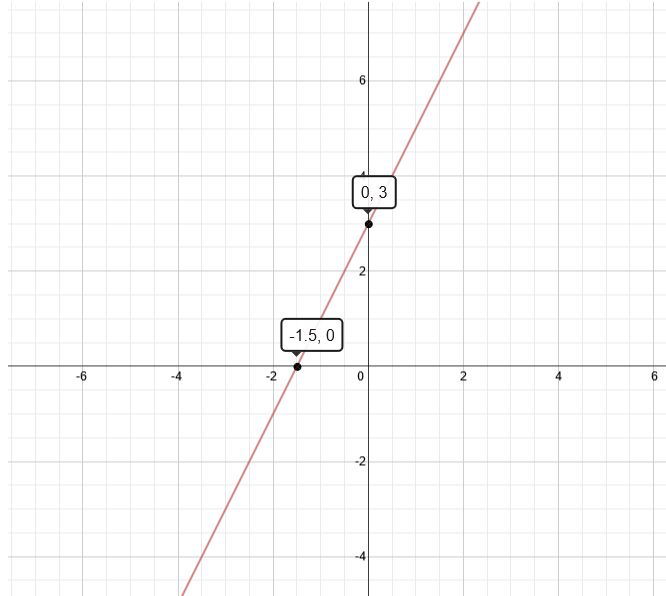
\includegraphics[scale=0.45]{graph.png}\\ \footnotesize{sample figure} 
%must set an empty line before and after, otherwise other text will be affected too
%\leftskip and \rightskip refer to flushleft and right

}
%format can also be \includegraphics[width=#/height=#]{*},  \includegraphics[angle=^]{*},

\section{Packages}
There are necessary to use packages while building a document. Packages can change or adjust the outline or looking of the document. Packages have to be downloaded from the MikTeX Console and install before applying to LaTeX. 
Packages can be imported by ``\textbackslash usepackage'' at the preamble, which is the blank area between ``documentclass'' and ``\bslash begin\{document\}''.
 %i.e. \usepackage{•}
 
\section{Colour}
You are able to change the colour of text using \textit{\textbf{colorx}} package. Just simply using command ``\bslash color\{color\}''. {\color{blue}{For Example, this is blue text.}} 

\section{Multi-Sources}
The format of using multi-sources rather than putting in one .tex file are as below. The sources should be in the same location.
\begin{align*}
&\text{ \textbackslash documentclass\{book\} }\\  % the document class ''book'' 
&\text{ \textbackslash includeonly\{chap1, appen1\} }\\ % only include 'chap1' and 'appen1' 
&\text{ \textbackslash begin\{document\} }\\
&\text{ \textbackslash include\{chap1\} }\\ % input chap1.tex 
&\text{ \textbackslash include\{chap2\} }\\ % input chap2.tex
&\text{ \textbackslash include\{chap3\} }\\ % input chap3.tex
&\text{ \textbackslash include\{appen1\} }\\ % input appen1.tex
&\text{ \textbackslash include\{appen2\} }\\ % input appen2.tex
&\text{ \textbackslash end\{document\} }
\end{align*}

\section{Sections}
Command: `\bslash parameter'\{`Title'\}\\
\begin{tabular}{|c|c|}
\hline
\textbf{Parameter} & \textbf{Priority} \\
\hline
part (in book and report) &Level -1 \\
\hline
part (in article ) &Level 0 \\
\hline
chapter (only in book and report) &Level 0 \\
\hline
section &Level 1 \\
\hline
subsection & Level 2 \\
\hline
subsubsection &Level 3 \\
\hline
paragraph &Level 4 \\
\hline
subparagraph &Level 5 \\
\hline
\end{tabular}
\clearpage
\section{Mathematics}
It is suggested to use`` \bslash frac'' instead of ``\bslash over'' in LxTeX.\\
Useful command: ``\bslash setlength\{\bslash mathindent\}\{0mm\}'' to set math mode indentation.
\subsection{Basic Maths symbols}
\begin{enumerate}
\item text: $\text{This is text in math mode instead of using mathrm}$ %\textrm, \textbf, etc are still work
\item math font: $D$, $\mathrm{D}, \mathnormal{D}$ %we also have \mathbf, \mathit, \mathtt, \mathbb, etc
\item textstyle and displaystyle: $\tfrac{1}{2}$ and $\dfrac{1}{2}$ , $\tbinom{n}{r}$ and $\dbinom{n}{r}$
%alternatively, you can add command '\textstyle' and '\displaystyle' instead of useing '\txxxx' nor '\dxxxx' 
\item approach to: ``\bslash approx'': $\approx$
\item limit: ``\bslash lim\_\{a \bslash to b\}''
\item integral: ``\bslash int'': $\int_a^b$
\item limits: ``\bslash limits'': place argument at top or bottom, e.g $\int \limits_a^b$
\item vectors: ``\bslash vec'': $\vec{v}$
\item summation: ``\bslash sum'': $\d{e^x=\sum_{n=0}^{\infty}\frac{x^n}{n!}}$
\item degree($\degree$): by `\textbf{\textit{gensymb}}' package: ``\bslash degree''
\end{enumerate}
\clearpage
\subsection{Equation array}
An equation array aims to group a set of equations. The format is as follows:\\
\bslash begin\{eqnarray\}\\
equation 1\\
equation 2\\
\vdots\\
equation n\\
\bslash end\{eqnarray\}\\
Sample output: 
\begin{eqnarray}
y &=& mx + c\\  %the ampersand sign '&' are different to that in align environment
x^2 + y^2 &=& 1
\end{eqnarray}

\subsection{Matrix withoit amsmath}%without 'amsmath'
You can make a matrix by array environment in mathematics environment. The following is the format:\\
\$ \bslash left( 
\bslash begin\{array\}\{clr\} {\scriptsize { *\{clr\} is the same as tabular}}\\
% {clr} refer to the alignment method from first column to last column, ie center, left and right, you can add as many as you can
	a\_\{11\} \& a\_\{12\} \& a\_\{13\}\\
	b\_\{21\} \& b\_\{22\} \& b\_\{23\}\\
	c\_\{31\} \& c\_\{32\} \& c\_\{33\}\\
\bslash end\{array\} \bslash right) \$ \\ % can use '$$'or '\[ \]' to make them centered
Output:
$  \left( 
\begin{array}{clr} 
	a_{11} & a_{12} & a_{13}\\
	b_{21} & b_{22} & b_{23}\\
	c_{31} & c_{32} & c_{33}
\end{array} \right) $ 

\subsection{Matrix with amsmath} %usepackage 'amsmath'
You can use \textit{\textbf{masmath}} package to easily build a matrix in matrix environment. There are ``matrix'', ``pmatrix'', ``bmatrix'', ``vmatrix'', ``Vmatrix'' and ``smallmatrix'' you can use. Below shows the sample outputs respectively. Note that ``smallmatrix'' is usually used to display matrix in a sentence.
$$
\begin{matrix} 
a & b \\
c & d 
\end{matrix} 
\quad
\begin{pmatrix}  
a & b \\
c & d 
\end{pmatrix}
\quad
\begin{bmatrix} 
a & b \\
c & d 
\end{bmatrix}
\quad
\begin{vmatrix} 
a & b \\
c & d 
\end{vmatrix}
\quad
\begin{Vmatrix} 
a & b \\
c & d 
\end{Vmatrix}
\quad
\begin{smallmatrix}  
  a&b\\
  c&d
\end{smallmatrix} 
$$
The matrices as show above are limited to 10 columns. If you want to use more than 10 columns, just adjust ``MaxMatrixCols'' to desired value, for example 15:
``\bslash setcounter{MaxMatrixCols}\{15\}''

\subsection{Alignment}
Environment enclosed by: \bslash begin\{align\} \dots \bslash end\{align\}.\\
The environment is automatically in math mode.\\
Using \& to be the indicator.\\
Example format:
\setlength{\mathindent}{0mm}
\begin{align*}
&\text{The resultant force:} &\overrightarrow{F_R} &= \overrightarrow{F_1} + \overrightarrow{F_2}\\
&&&= \{-4\vec{i}+2\vec{j}-3\vec{k}\} + \{3\vec{i}-4\vec{j}-2\vec{k} \} \\
&&&= \underline{ \underline{ \{-\vec{i}-2\vec{j}-5\vec{k}\} }} \ \mathrm{kN} \\[0.5cm]
&\text{The distance of OA:} &\overrightarrow{r_{OA}} &= \{3\vec{i}-0.12\vec{j}+0.2\vec{k} \} \  \mathrm{m} \\
&\text{The distance of OB:} &\overrightarrow{r_{OB}} &= \{3\vec{i}+0.12\vec{j}+0.2\vec{k} \} \  \mathrm{m} \\
&\text{Moment at point O:} &\overrightarrow{M_O} &= \sum{ (\vec{r} \times \vec{F} ) }\\
&&&= \{3\vec{i}-0.12\vec{j}+0.2\vec{k} \}  \times \{-4\vec{i}+2\vec{j}-3\vec{k} \} 
   + \{3\vec{i}+0.12\vec{j}+0.2\vec{k} \} \times \{3\vec{i}-4\vec{j}-2\vec{k} \} \\
&&&= \underline{\underline{ \{ -0.2\vec{i} - 3.2\vec{j} - 6.84\vec{k} \} }}\  \mathrm{kNm}
\end{align*}
\end{document}